%
%   latex writeup for Peerchat
%   6.858 Final Project
%   December 2013
%   forrestp, ameeshg, kseibert, cbieden
%
%

\documentclass{article}

\usepackage{geometry}
\geometry{letterpaper}

\usepackage{doc}

\usepackage{graphicx}
%\usepackage{float}
%\usepackage{caption}
%\usepackage{subcaption}

%\usepackage{epstopdf}

%\usepackage{enumitem}
%\setdescription{leftmargin=\parindent,labelindent=1cm}

\title{Peerchat: a Distributed, P2P Communication Network based on Kademlia}
\author{
  Forrest Pieper\\
  Will Drevo\\
  Colin Taylor
}
\date{May 4th, 2014}

\begin{document}

\maketitle

\section{Motivation}
\label{Motivation}

What we today know as the "internet" was started as a US DARPA military project, a network of nodes distributed geographically across the US in order to ensure fault tolerance in the case of a nuclear attack \cite{?}. Today, ironically, many feel the internet has become too centralized. \\

\section{Introduction}

\textit{Peerchat} is a distributed, P2P chat system based on the Kademlia DHT \cite{Maymounkov02} system.

In Peerchat, each client, or user, creates a Kademlia node with a 64 int Node ID created from the hash of its IP address. Users find each other by storing a username -> Ip Address mapping in the distributed hash table (DHT). It does so by storing this map at the nearest K closest nodes to the hash of the username. Users call PeerChat's FindUser(username) API, which returns the IP address. Using Kademlia ensures that user?s find each other using at most log(n) hops, where n is the number of nodes (assuming the routing tables are filled in each bucket). 

A user tries to send a message directly, using a background process that keeps sending pending messages until a node replies. In the case of failure, a node also sends the message to the K nearest nodes around the node, which add the message to their background queues. In this way, if the original sender logs out, and the recipient logs back in, the recipient can still receive the message. We call this functionality offline chat.

We implemented two main clerks - Users and Nodes. A user contains the API which our Client code uses directly. A user has a username, an Ip address, a message history etc. A user actually sends messages to another user. It also has a pointer to a Node. In this way, a user uses kademlia to find other users's IP addresses and to send offline messages.

A node is a Kademlia node as described in the protocol. It is a standalone system which implements it?s 4 main functions: StoreUser, FindNode, FindUser and Ping. It 

\section{Background and Related Work}

A very similar effort is BitTorrent Chat \cite{?}. 

\section{System}

Below is a diagram of a single Peerchat node. 

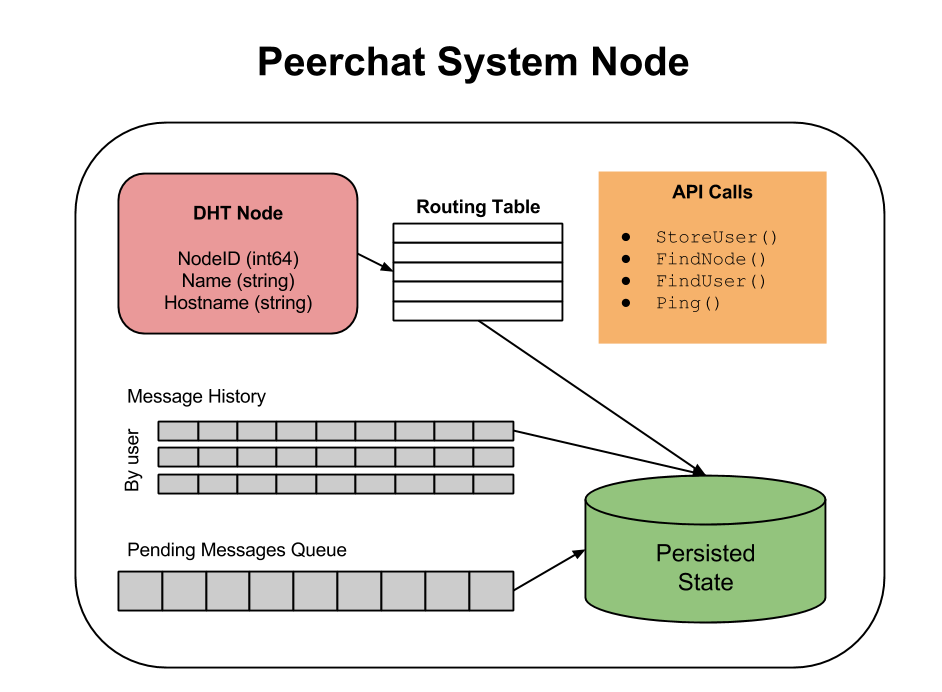
\includegraphics[scale=0.5]{peerchat}

The system is parameterized by the normal Kademlia settings of $k$ and $\alpha$, however has a number of marked differences to make it adaptable to a system where users must persist by their usernames when connecting on different IP addresses (though not different hard disks). 

A Peerchat user consists of a number of different routines all working together. A short description of their function is below:

Separate threads (goroutines):
\begin{enumerate}
	\item Message Queuing \\
	The message queuing routine is what acts when a user submits a message. The user?s node sends the message to a queue where it is stored until the Message Sender can deal with the message. Additionally, messages that are being forwarded on in the case of offline messaging are also ?piggybacked? into other user?s pending messages queue, and await being forwarded to other nodes. 

	\item Message Sender \\
	The Message Sending goroutine iterates through the list of recipients with messages to be sent in the User?s queues.  Next, using the DHT, the Message Sender attempts to locate and ping the recipient peer. If the peer is online, the message is sent directly through TCP using an RPC call. If the peer is offline, the Message is sent to the K closest neighbors in the DHT by the XOR metric to increase the chances of message delivery when the recipient happens to come online. 

	\item Connection Acceptor \\
The connection acceptor is the Peerchat routine that accepts RPC requests and spins off new goroutines to service them. 

	\item Periodic Backup \\
	As well as backing up the system after each received message, Peerchat also backs up it?s message history, routing table, received and seen messages maps, and connection information every 30 seconds. This covers for unpopular nodes who are more often message ?forwarders? than receivers while avoiding spurious serializations to disk. 
\end{enumerate}

\subsection{Persistence}

We persist nodes' state by periodically serializing a user's routing table and messaging log to disk. 

\subsection{Offline Usage}

\section{Demonstration}

\subsection{User Registration}
\subsection{User Login}
\subsection{Correctness Testing}
\subsection{Performance Testing}

\section{Future Work}

Security?

\section{Conclusion}

Peerchat is the best, blah, blah.

\begin{thebibliography}{99}
  \bibitem{Maymounkov02}
    %Kademlia paper
   Maymounkov, Petar and David Mazieres
   ''Kademlia: A Peer-to-peer Information System Based on the XOR Metric''
   \textit{Peer-to-Peer Systems. Springer Berlin Heidelberg}, 2002. 53-65
 
\end{thebibliography}

\end {document}
